% 0067(본책 17쪽) — 좌표평면에 직선 y=(5/2)x+5 의 그래프(x축 양의 방향과 이루는 각 a). 라벨: x·y·O·a·식. 절편 값은 원문에 없으므로 적지 않는다. 스캔 삽화를 TikZ 로 다시 그림.
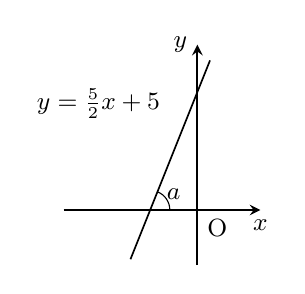
\begin{tikzpicture}[scale=1, line width=0.5pt]
  \draw[->, >=stealth, line width=0.7pt] (-1.7,0) -- (0.8,0) node[below, font=\small] {$x$};
  \draw[->, >=stealth, line width=0.7pt] (0,-0.7) -- (0,2.1) node[left, font=\small] {$y$};
  \node[font=\small, below right] at (0,0) {O};
  \draw[line width=0.6pt] (-0.85,-0.625) -- (0.16,1.9);
  % 각 a(점 (-0.6,0) 에서 x축 양의 방향과 직선 사이)
  \draw[line width=0.4pt] (-0.35,0) arc[start angle=0, end angle=68.2, radius=0.25cm];
  \node[font=\small] at (-0.3,0.2) {$a$};
  \node[font=\small, left] at (-0.35,1.35) {$y=\frac{5}{2}x+5$};
\end{tikzpicture}
